% !TEX program = xelatex
\documentclass[UTF8,zihao=-4,oneside,openany]{ctexbook}

% Shared style for the combined handout.  Section files keep standalone
% preambles for now, while the master document uses this single definition.
\usepackage[a4paper,top=20mm,bottom=22mm,left=19mm,right=19mm,headheight=24pt]{geometry}
\usepackage[table]{xcolor}
\usepackage{amsmath,amssymb,mathtools,bm}
\usepackage{siunitx}
\usepackage{booktabs,tabularx,array,multicol}
\usepackage{enumitem}
\usepackage{tikz}
\usetikzlibrary{arrows.meta,positioning,calc,angles,quotes,patterns}
\usepackage[most]{tcolorbox}
\usepackage{fancyhdr}
\usepackage{hyperref}

\definecolor{Ink}{HTML}{202326}
\definecolor{DeepBlue}{HTML}{294E69}
\definecolor{Blue}{HTML}{47687D}
\definecolor{PaleBlue}{HTML}{F3F5F6}
\definecolor{Gold}{HTML}{6E777D}
\definecolor{PaleGold}{HTML}{F6F6F5}
\definecolor{Green}{HTML}{5B6D76}
\definecolor{PaleGreen}{HTML}{F3F5F6}
\definecolor{Alert}{HTML}{666B6F}
\definecolor{PaleAlert}{HTML}{F6F6F6}
\definecolor{RuleGray}{HTML}{D3D7DA}
\definecolor{TextGray}{HTML}{61686D}
\definecolor{SoftGray}{HTML}{F6F6F6}

\color{Ink}
\sisetup{
  per-mode=symbol,
  inter-unit-product=\ensuremath{{}\cdot{}},
  exponent-product=\times
}

\hypersetup{
  colorlinks=true,
  linkcolor=DeepBlue,
  urlcolor=Blue,
  pdfsubject={高中物理竞赛一轮资料重排讲义},
  pdfauthor={物理竞赛一轮资料编写组}
}

\setlength{\parindent}{2em}
\setlength{\parskip}{0.25em}
\setlist{nosep,leftmargin=2em}
\setcounter{secnumdepth}{3}
\setcounter{tocdepth}{2}
\numberwithin{equation}{section}
\counterwithin{table}{section}
\allowdisplaybreaks[2]
\emergencystretch=2em

\ctexset{
  chapter={
    format=\raggedright\LARGE\bfseries\color{Ink},
    titleformat=\LARGE\bfseries\color{Ink},
    beforeskip=0pt,
    afterskip=18pt
  },
  section={
    format=\Large\bfseries\color{DeepBlue},
    beforeskip=1.8ex,
    afterskip=1.0ex
  },
  subsection={
    format=\large\bfseries\color{Ink},
    beforeskip=1.5ex,
    afterskip=0.8ex
  },
  subsubsection={format=\normalsize\bfseries\color{Ink}}
}

\pagestyle{fancy}
\fancyhf{}
\fancyhead[L]{\small\color{TextGray}高中物理竞赛一轮讲义}
\fancyhead[R]{\small\color{TextGray}第一章\quad 数学与物理工具}
\fancyfoot[C]{\small\color{TextGray}\thepage}
\renewcommand{\headrulewidth}{0.4pt}
\renewcommand{\headrule}{\hbox to\headwidth{\color{RuleGray}\leaders\hrule height \headrulewidth\hfill}}

\newcommand{\dimens}[1]{\operatorname{dim}\!\left(#1\right)}
\newcommand{\dd}{\mathop{}\!\mathrm{d}}
\newcommand{\vect}[1]{\bm{#1}}
\newcommand{\uvec}[1]{\hat{\vect{#1}}}
\newcommand{\e}{\mathrm e}
\newcommand{\order}[1]{\mathcal O\!\left(#1\right)}
\DeclareMathOperator{\proj}{proj}
\newcommand{\examplesource}[1]{%
  \par{\small\color{TextGray}题源：#1}\par
}

\newtcolorbox{goalbox}{
  enhanced,breakable,
  colback=PaleBlue,colframe=Blue,
  boxrule=0.7pt,arc=2mm,
  title={本节目标},fonttitle=\bfseries,
  coltitle=DeepBlue,
  attach boxed title to top left={xshift=5mm,yshift=-2mm},
  boxed title style={colback=white,colframe=Blue,boxrule=0.7pt,arc=1.5mm}
}

\newtcolorbox{sourcebox}{
  enhanced,breakable,
  colback=SoftGray,colframe=RuleGray,
  boxrule=0.5pt,arc=0mm,
  title={题源说明},fonttitle=\bfseries,
  coltitle=Ink,colbacktitle=SoftGray,
  borderline west={1.2pt}{0pt}{TextGray}
}

\newtcolorbox[auto counter,number within=section]{examplebox}[2][]{
  enhanced,breakable,
  colback=white,colframe=RuleGray,
  boxrule=0.5pt,arc=0mm,
  title={例题~\thetcbcounter\quad #2},fonttitle=\bfseries,
  coltitle=Ink,colbacktitle=PaleBlue,
  borderline west={1.4pt}{0pt}{DeepBlue},
  #1
}

\newtcolorbox{methodbox}[1]{
  enhanced,breakable,
  colback=PaleBlue,colframe=RuleGray,
  boxrule=0.5pt,arc=0mm,
  title={方法：#1},fonttitle=\bfseries,
  coltitle=Ink,colbacktitle=PaleBlue,
  borderline west={1.2pt}{0pt}{DeepBlue}
}

\newtcolorbox{warningbox}[1]{
  enhanced,breakable,
  colback=SoftGray,colframe=RuleGray,
  boxrule=0.5pt,arc=0mm,
  title={易错提醒：#1},fonttitle=\bfseries,
  coltitle=Ink,colbacktitle=SoftGray,
  borderline west={1.2pt}{0pt}{TextGray}
}

\newtcolorbox{extensionbox}[1]{
  enhanced,breakable,
  colback=PaleGold,colframe=Gold,
  boxrule=0.5pt,arc=0mm,
  title={拓展：#1},fonttitle=\bfseries,
  coltitle=Ink,colbacktitle=PaleGold,
  borderline west={1.2pt}{0pt}{DeepBlue}
}

\newtcolorbox{summarybox}{
  enhanced,breakable,
  colback=PaleBlue,colframe=DeepBlue,
  boxrule=0.9pt,arc=1.5mm,
  title={本节小结},fonttitle=\bfseries,
  coltitle=white,colbacktitle=DeepBlue
}

\newtcolorbox{exercisebox}[1]{
  enhanced,breakable,
  colback=white,colframe=RuleGray,
  boxrule=0.7pt,arc=1.5mm,
  title={#1},fonttitle=\bfseries,
  coltitle=DeepBlue,colbacktitle=PaleBlue
}

\tikzset{
  vector/.style={-{Latex[length=2.5mm]},very thick,draw=DeepBlue},
  component/.style={-{Latex[length=2.2mm]},thick,draw=TextGray},
  axis/.style={-{Latex[length=2mm]},thin,draw=TextGray},
  guide/.style={densely dashed,draw=TextGray},
  curve/.style={very thick,draw=DeepBlue},
  tangent/.style={thick,draw=TextGray},
  secant/.style={thick,draw=DeepBlue}
}

\usetikzlibrary{decorations.pathmorphing,decorations.markings,intersections,calc,arrows.meta,positioning,patterns,shapes.geometric}

\newcommand{\Needspace}[1]{%
  \par
  \ifdim\dimexpr\pagegoal-\pagetotal\relax<#1\relax
    \newpage
  \fi
}

\newtcolorbox{origexamplebox}[1]{
  enhanced,breakable,
  colback=white,colframe=RuleGray,
  boxrule=0.5pt,arc=0mm,
  title={#1},fonttitle=\bfseries,
  coltitle=Ink,colbacktitle=PaleBlue,
  borderline west={1.4pt}{0pt}{DeepBlue}
}

\NewDocumentEnvironment{xesolution}{+b}{%
  \par\smallskip
  \begingroup\small
  \noindent{\bfseries\color{DeepBlue}解答}\quad #1
  \par\endgroup\medskip
}{}

\hypersetup{
  pdftitle={高中物理竞赛一轮讲义：第31节 相变（含解答与解图）},
  pdfsubject={依据学而思兴趣一阶热物理第22讲完整整理，并补写推导、解答与解图},
  pdfauthor={原题资料：学而思；整理与解答：物理竞赛一轮资料编写组}
}

\fancyhead[R]{\small\color{TextGray}寒假兴趣一阶\quad 第 22 讲}
\renewcommand{\theequation}{22.\arabic{equation}}

% All annotations are transparent: labels never carry an opaque rectangular mask.
\tikzset{
  xeslabel/.style={font=\small,text=Ink,fill=none,inner sep=0.6pt},
  xessmall/.style={font=\footnotesize,text=TextGray,fill=none,inner sep=0.5pt},
  xesline/.style={draw=Ink,line width=0.85pt},
  xesblue/.style={draw=DeepBlue,line width=1.05pt},
  xesarrow/.style={-{Latex[length=2.2mm,width=1.4mm]},draw=DeepBlue,line width=0.9pt},
  forcearrow/.style={-{Latex[length=2.3mm,width=1.5mm]},draw=DeepBlue,line width=1.0pt}
}

\newcommand{\diagramcaption}[1]{%
  \par\vspace{-0.25em}
  \begin{center}\small\color{TextGray}#1\end{center}
  \vspace{0.3em}
}

\newcommand{\phaseDiagramWater}{%
\begin{center}
\begin{tikzpicture}[x=1.03cm,y=0.73cm]
  \draw[xesline,-{Latex[length=2mm]}] (0,0)--(8.7,0) node[xeslabel,below left=1pt] {$T$};
  \draw[xesline,-{Latex[length=2mm]}] (0,0)--(0,6.2) node[xeslabel,below right=1pt] {$p$};
  \coordinate (A) at (2.55,1.55);
  \coordinate (C) at (7.05,4.35);
  \draw[xesblue] (0.25,0.35) .. controls (0.95,0.7) and (1.75,1.15) .. (A);
  \draw[xesblue] (A) .. controls (4.0,1.9) and (5.65,3.0) .. (C);
  \draw[xesblue] (A) .. controls (2.25,3.15) and (1.92,4.75) .. (1.7,5.9);
  \fill[DeepBlue] (A) circle (1.4pt) (C) circle (1.4pt);
  \node[xeslabel,anchor=south east] at ($(A)+(-0.08,0.05)$) {$A$};
  \node[xeslabel,anchor=south west] at ($(C)+(0.08,0.04)$) {$C$};
  \node[xessmall,align=center] at (1.35,3.35) {固态};
  \node[xessmall,align=center] at (4.1,3.8) {液态};
  \node[xessmall,align=center] at (5.55,1.15) {气态};
  \node[xessmall] at (4.75,3.25) {汽化曲线};
  \node[xessmall] at (.5,-.75) {升华曲线};
  \draw[RuleGray,->] (.5,-.5)--(.85,.67);
  \node[xessmall,rotate=79] at (2.8,4.65) {熔化曲线};
  \draw[RuleGray,densely dashed] (A)--(2.55,0) node[xessmall,below,align=center] {$0.01\,{}^{\circ}\mathrm C$};
  \draw[RuleGray,densely dashed] (A)--(0,1.55) node[xessmall,left] {$611.73\,\mathrm{Pa}$};
  \draw[RuleGray,densely dashed] (C)--(7.05,0) node[xessmall,below] {$374\,{}^{\circ}\mathrm C$};
  \draw[RuleGray,densely dashed] (C)--(0,4.35) node[xessmall,left,align=right] {$2.2\times10^7\,\mathrm{Pa}$};
  \node[xessmall,anchor=south] at (7.05,4.95) {临界点};
  \node[xessmall,anchor=west] at (2.72,1.18) {三相点};

  % microscopic phase sketches, placed away from the curves
  \begin{scope}[shift={(8.0,1.1)},scale=0.58]
    \draw[RuleGray,rounded corners=2pt] (-0.75,-0.75) rectangle (0.75,0.75);
    \foreach \x in {-0.48,0,0.48}\foreach \y in {-0.48,0,0.48}{\fill[DeepBlue!70] (\x,\y) circle (1.1pt);}
    \node[xessmall] at (0,-1.05) {固};
  \end{scope}
  \begin{scope}[shift={(8.0,2.45)},scale=0.58]
    \draw[RuleGray,rounded corners=2pt] (-0.75,-0.75) rectangle (0.75,0.75);
    \foreach \p in {(-.5,-.35),(-.05,-.48),(.42,-.25),(-.4,.15),(.08,.06),(.5,.3),(-.15,.48)}{\fill[DeepBlue!70] \p circle (1.1pt);}
    \node[xessmall] at (0,-1.05) {液};
  \end{scope}
  \begin{scope}[shift={(8.0,3.8)},scale=0.58]
    \draw[RuleGray,rounded corners=2pt] (-0.75,-0.75) rectangle (0.75,0.75);
    \foreach \p in {(-.53,-.48),(.48,-.31),(-.18,.08),(.45,.5),(-.5,.43)}{\fill[DeepBlue!70] \p circle (1.1pt);}
    \node[xessmall] at (0,-1.05) {气};
  \end{scope}
\end{tikzpicture}
\end{center}}





\newcommand{\criticalApparatusFigure}{%
\begin{center}
\includegraphics[width=.83\linewidth]{/Users/dongxingxi/Documents/物理竞赛一轮资料/sample/xes-original/restructured-complete/assets/ch17/critical-cell.png}\par\smallskip
\begin{tikzpicture}[x=1cm,y=1cm]
  \foreach \dx in {0,4,8}{
    \draw[Ink,line width=1pt,rounded corners=7pt] (\dx,0) rectangle +(2.5,3.35);
    \draw[RuleGray,line width=2.2pt] (\dx+.28,.25)--(\dx+.28,3.1);
  }
  % below critical: two visibly separated phases
  \fill[DeepBlue!12] (.08,.08) rectangle (2.42,1.48);
  \draw[DeepBlue,line width=1.1pt] (.08,1.48)--(2.42,1.48);
  \foreach \p in {(.45,.45),(.82,.72),(1.18,.38),(1.62,.72),(2.05,.42),(.55,1.05),(1.45,1.08),(2.1,1.1)}{\fill[DeepBlue!65] \p circle (1.2pt);}
  \foreach \p in {(.65,2.1),(1.75,2.65),(2.05,2.0)}{\fill[DeepBlue!50] \p circle (1.0pt);}
  \node[xessmall,align=center] at (1.25,-.48) {$T<T_c$\\清晰气液界面};
  % critical opalescence: fluctuating cloudy density
  \foreach \p/\r in {(4.45,.45)/.18,(4.8,1.0)/.25,(5.35,.62)/.3,(5.9,1.25)/.22,(4.55,1.75)/.35,(5.25,1.65)/.2,(5.8,2.1)/.32,(4.85,2.55)/.28,(5.65,2.85)/.22}{
    \shade[inner color=DeepBlue!28,outer color=white] \p circle (\r);
  }
  \draw[DeepBlue!60,densely dotted] (4.15,1.5) .. controls (4.8,1.7) and (5.5,1.25) .. (6.35,1.55);
  \node[xessmall,align=center] at (5.25,-.48) {$T\approx T_c$\\临界乳光};
  % above critical: uniform supercritical fluid
  \fill[DeepBlue!8] (8.08,.08) rectangle (10.42,3.19);
  \foreach \p in {(8.45,.45),(8.85,.85),(9.35,.42),(9.9,.75),(8.55,1.35),(9.15,1.55),(9.8,1.25),(8.7,2.1),(9.35,2.25),(10,2.05),(8.45,2.75),(9.05,2.95),(9.75,2.7)}{\fill[DeepBlue!45] \p circle (1.05pt);}
  \node[xessmall,align=center] at (9.25,-.48) {$T>T_c,\ p>p_c$\\均匀超临界流体};
\end{tikzpicture}
\end{center}}

% Quantitative diagrams: shared formulas determine points and curves.
\newcommand{\vdWIsotherms}{%
\begin{center}\begin{tikzpicture}
\begin{axis}[width=.82\linewidth,height=6cm,axis lines=left,xmin=.48,xmax=3.5,ymin=0,ymax=2.7,
xlabel={$v'=V/V_c$},ylabel={$p'=p/p_c$},xtick={1,2,3},ytick={1,2},clip=true]
\foreach \t in {.85,.9,1,1.08,1.16,1.24}{
\addplot[DeepBlue,domain=.48:3.3,samples=250]{8*\t/(3*x-1)-3/x^2};}
\addplot[only marks,mark=*,mark size=1.3pt] coordinates{(1,1)};
\node[above right] at (axis cs:1.02,1.04) {$C$};
\draw[dashed,TextGray] (axis cs:1,0)--(axis cs:1,1);
\node[align=left,anchor=north east,font=\small] at (axis cs:3.35,2.5)
{$t'=0.85,\ 0.90,\ 1.00,$\\$1.08,\ 1.16,\ 1.24$\\从下向上};
\end{axis}\end{tikzpicture}\end{center}}

\newcommand{\criticalPointFigure}{%
\begin{center}\begin{tikzpicture}
\begin{axis}[width=6cm,height=5.3cm,axis lines=left,xmin=.55,xmax=2.3,ymin=0,ymax=2.4,
xlabel={$v'$},ylabel={$p'$},xtick={1,2},ytick={1,2}]
\addplot[DeepBlue,thick,domain=.56:2.2,samples=250]{8/(3*x-1)-3/x^2};
\addplot[only marks,mark=*] coordinates{(1,1)};
\draw[dashed,TextGray] (axis cs:.8,1)--(axis cs:1.3,1);
\node[above right] at (axis cs:1.07,1.1) {$C$};
\end{axis}
\begin{scope}[xshift=7cm,x=.88cm,y=.82cm]
\draw[axis] (0,0)--(5.7,0) node[right]{$T$};
\draw[axis] (0,0)--(0,5.5) node[above]{$p$};
\draw[DeepBlue,thick,domain=.6:4,samples=100] plot(\x,{.2+.2*\x*\x});
\coordinate (P) at (1,1.5);\coordinate (M) at (2.54951,1.5);\coordinate (Q) at (5,1.5);
\coordinate (A) at (1,4.6);\coordinate (B) at (5,4.6);\coordinate (C) at (4,3.4);
\draw[->,Ink] (P)--(M);\draw[->,Ink] (M)--(Q);
\draw[->,DeepBlue,dashed] (P)--(A);\draw[->,DeepBlue,dashed] (A)--(B);\draw[->,DeepBlue,dashed] (B)--(Q);
\foreach \q in {P,M,Q,A,B,C}{\fill (\q) circle(1.2pt);}
\foreach \q in {P,M,Q}{\node[below=4pt] at (\q){$\q$};}
\foreach \q in {A,B,C}{\node[above=4pt] at (\q){$\q$};}
\node[font=\small] at (2.2,3.7){液相};\node[font=\small] at (4.7,.55){气相};
\end{scope}
\node[font=\small] at (2.5,-1) {(a) 临界等温线};
\node[font=\small] at (9,-1) {(b) 穿越与绕行路径};
\end{tikzpicture}\end{center}}

\newcommand{\maxwellAreaFigure}{%
\begin{center}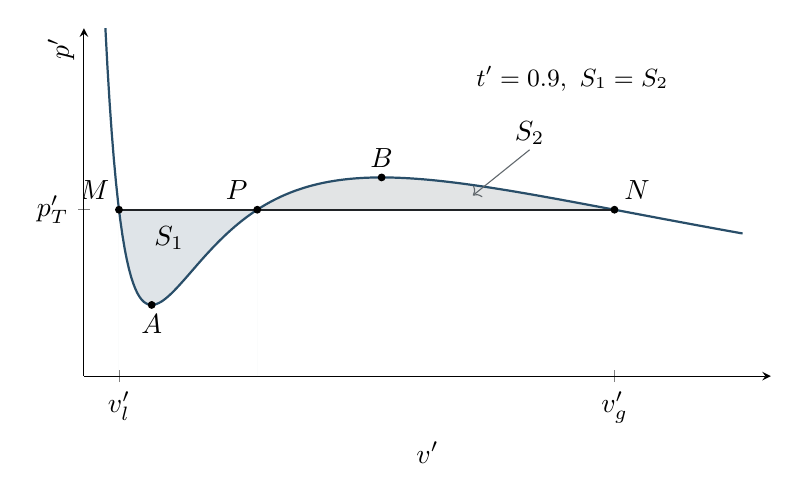
\begin{tikzpicture}
\begin{axis}[width=.85\linewidth,height=6cm,axis lines=left,xmin=.48,xmax=2.9,ymin=.25,ymax=1.08,
xlabel={$v'$},ylabel={$p'$},ylabel style={at={(axis description cs:0,1)},anchor=south east},xtick={.603402,2.348842},xticklabels={$v_l'$,$v_g'$},ytick={.64699835},yticklabels={$p_T'$}]
\addplot[draw=none,fill=DeepBlue!15,domain=.603401903:1.090526633,samples=120]
{7.2/(3*x-1)-3/x^2} -- (axis cs:1.090526633,.646998352)--(axis cs:.603401903,.646998352)\closedcycle;
\addplot[draw=none,fill=Gold!20,domain=1.090526633:2.348842376,samples=120]
{7.2/(3*x-1)-3/x^2} -- (axis cs:2.348842376,.646998352)--(axis cs:1.090526633,.646998352)\closedcycle;
\addplot[DeepBlue,thick,domain=.54:2.8,samples=300]{7.2/(3*x-1)-3/x^2};
\draw[Ink,thick] (axis cs:.603401903,.646998352)--(axis cs:2.348842376,.646998352);
\addplot[only marks,mark=*,mark size=1.2pt] coordinates{(.603402,.646998)(.718597,.419843)(1.090527,.646998)(1.528505,.724013)(2.348842,.646998)};
\node[above left] at (axis cs:.603402,.646998){$M$};
\node[below] at (axis cs:.718597,.419843){$A$};
\node[above left] at (axis cs:1.090527,.646998){$P$};
\node[above] at (axis cs:1.528505,.724013){$B$};
\node[above right] at (axis cs:2.348842,.646998){$N$};
\node at (axis cs:.78,.58){$S_1$};\node at (axis cs:2.05,.83){$S_2$};
\draw[->,TextGray] (axis cs:2.05,.79)--(axis cs:1.85,.681);
\node[font=\small] at (axis cs:2.2,.96){$t'=0.9,\ S_1=S_2$};
\end{axis}\end{tikzpicture}\end{center}}

\newcommand{\contrailFigure}{%
\begin{center}\includegraphics[width=.88\linewidth]{/Users/dongxingxi/Documents/物理竞赛一轮资料/sample/xes-original/restructured-complete/assets/ch17/contrail.png}\end{center}}

\newcommand{\mercuryTubeFigure}{%
\begin{center}\begin{tikzpicture}[x=.17cm,y=.17cm]
\draw[Ink,thick] (0,5)--(0,10)--(31,10) (0,5)--(31,5);
\fill[DeepBlue!25] (17,5.1) rectangle(27,9.9);
\draw[DeepBlue] (17,5)--(17,10) (27,5)--(27,10);
\draw[<->] (0,2)--(17,2) node[midway,below,font=\small]{$17\,\mathrm{cm}$};
\draw[<->] (17,13)--(27,13) node[midway,above,font=\small]{$10\,\mathrm{cm}$};
\node[font=\small] at (22,7.5){Hg};
\node[font=\small,align=center] at (8.5,18){封闭气体\\空气与饱和汞蒸气};
\draw[->,TextGray] (8.5,15)--(8.5,9);
\draw[Ink,thick] (47,0)--(47,33)--(52,33)--(52,0);
\fill[DeepBlue!25] (47.1,3) rectangle(51.9,13);
\draw[DeepBlue] (47,3)--(52,3) (47,13)--(52,13);
\node[font=\small] at (49.5,8){Hg};
\draw[<->] (56,13)--(56,33) node[midway,right,font=\small]{$20\,\mathrm{cm}$};
\draw[<->] (56,3)--(56,13) node[midway,right,font=\small]{$10\,\mathrm{cm}$};
\node[font=\small,align=center] at (37,26){同温度的\\封闭气体};
\draw[->,TextGray] (44,24)--(48,24);
\node[below,font=\small] at (49.5,0){开口，外接大气};
\node[above,font=\small] at (49.5,34){封闭端};
\end{tikzpicture}\end{center}}

\newcommand{\mixedGasPVFigure}{%
\begin{center}\begin{tikzpicture}
\begin{axis}[width=.8\linewidth,height=5.7cm,axis lines=left,xmin=0,xmax=4.6,ymin=0,ymax=5.7,
xlabel={$x=V'/V$},ylabel={$p/\mathrm{atm}$},xtick={.5,1,2,4},ytick={1,2,3,5}]
\addplot[DeepBlue,thick,domain=.45:2,samples=150]{1+2/x};
\addplot[DeepBlue,thick,dashed,domain=2:4.4,samples=120]{4/x};
\addplot[only marks,mark=*] coordinates{(.5,5)(1,3)(2,2)(4,1)};
\draw[dotted] (axis cs:2,0)--(axis cs:2,2);
\node[align=left,font=\small] at (axis cs:3.2,4.3){$x<2$：液体仍在\\$x\ge2$：水全汽化};
\node[above right,font=\small] at (axis cs:2,2.1){液体刚好消失};
\end{axis}\end{tikzpicture}\end{center}}

\newcommand{\pressureCookerQuestionFigure}{%
\begin{center}\begin{tikzpicture}
\begin{scope}[x=.6cm,y=.6cm]
\fill[DeepBlue!15] (.05,.05) rectangle(3.95,1.7);
\draw[thick] (0,4)--(0,0)--(4,0)--(4,4);
\draw[thick] (-.2,4)--(1.7,4)--(1.7,4.6) (2.3,4.6)--(2.3,4)--(4.2,4);
\draw[thick,fill=gray!15] (1.4,4.65) rectangle(2.6,5.15);
\draw[DeepBlue] (0,1.7)--(4,1.7);
\node[font=\small,above] at (2,5.3){限压阀 $S$};
\node[font=\small] at (2,2.6){气相};
\node[font=\small] at (2,.8){液态水};
\end{scope}
\begin{axis}[at={(3.6cm,0)},anchor=south west,width=8cm,height=5.0cm,axis lines=left,
xmin=0,xmax=130,ymin=0,ymax=260,xlabel={$t/{}^\circ\mathrm C$},ylabel={$p_w/\mathrm{kPa}$},
xtick={10,30,50,70,90,100,120},ytick={0,50,100,150,200,250},grid=both,
minor tick num=1,grid style={draw=RuleGray!70},tick label style={font=\scriptsize}]
\addplot[DeepBlue,thick] table[x=t,y=ps]{assets/ch17/saturation.dat};
\end{axis}\end{tikzpicture}\end{center}}

\newcommand{\pressureCookerFigure}{%
\begin{center}\begin{tikzpicture}
\begin{scope}[x=.7cm,y=.7cm]
\fill[DeepBlue!15] (.05,.05) rectangle(3.95,1.7);
\draw[thick] (0,4)--(0,0)--(4,0)--(4,4);
\draw[thick] (-.2,4)--(1.7,4)--(1.7,4.6) (2.3,4.6)--(2.3,4)--(4.2,4);
\draw[thick,fill=gray!15] (1.4,4.65) rectangle(2.6,5.15);
\draw[DeepBlue] (0,1.7)--(4,1.7);
\draw[->,DeepBlue] (2,3.2)--(2,4.5);
\draw[->,DeepBlue] (1.7,4.63)--(.7,4.63);
\node[font=\small,above] at (2,5.3){限压阀 $S$};
\node[font=\small,align=center] at (2,2.4){空气与水蒸气};
\node[font=\small] at (2,.8){液态水};
\end{scope}
\begin{axis}[at={(4.2cm,0)},anchor=south west,width=8cm,height=5.8cm,axis lines=left,
xmin=0,xmax=130,ymin=0,ymax=340,xlabel={$t/{}^\circ\mathrm C$},ylabel={$p/\mathrm{kPa}$},
xtick={10,90,120},ytick={100,200,300},legend style={at={(.02,.98)},anchor=north west,font=\scriptsize,draw=none,fill=none}]
\addplot[DeepBlue,thick] table[x=t,y=ps]{assets/ch17/saturation.dat};\addlegendentry{$p_w$}
\addplot[TextGray,dashed] table[x=t,y=pa]{assets/ch17/saturation.dat};\addlegendentry{$p_a$（封闭外推）}
\addplot[Ink,thick,restrict x to domain=0:90.174448744] table[x=t,y=total]{assets/ch17/saturation.dat};\addlegendentry{$p_a+p_w$（开启前）}
\addplot[Ink,dashed,restrict x to domain=90.174448744:130] table[x=t,y=total]{assets/ch17/saturation.dat};
\addplot[Ink,thick,domain=90.174448744:120]{198.671424787};
\addplot[dotted,domain=0:128]{198.671424787};
\addplot[only marks,mark=*] coordinates{(90.174448744,198.671424787)(120,198.671424787)};
\draw[dotted] (axis cs:90.174448744,0)--(axis cs:90.174448744,198.671424787)
(axis cs:120,0)--(axis cs:120,198.671424787);
\node[font=\small,anchor=north] at (axis cs:109,191){$p_*$};
\end{axis}\end{tikzpicture}\end{center}}

\newcommand{\twoVesselsFigure}{%
\begin{center}\begin{tikzpicture}[x=1cm,y=1cm]
\fill[DeepBlue!12] (7.22,.02) rectangle(10.38,.95);
\draw[thick] (3.2,1.5)--(3.2,0)--(0,0)--(0,3.45)--(3.2,3.45)--(3.2,1.9);
\draw[thick] (7.2,1.5)--(7.2,0)--(10.4,0)--(10.4,3.45)--(7.2,3.45)--(7.2,1.9);
\draw[thick] (3.2,1.5)--(7.2,1.5) (3.2,1.9)--(7.2,1.9);
\draw[DeepBlue] (7.2,.95)--(10.4,.95);
\node[font=\small,above] at (5.2,2.15){连通细管};
\node[align=center] at (1.6,2.6){热端\\$100{}^\circ\mathrm C$};
\node[align=center] at (8.8,2.6){冷端\\$0{}^\circ\mathrm C$};
\node[font=\small] at (8.8,.45){凝结水};
\draw[->,DeepBlue] (4.2,.9)--(6.2,.9);
\node[font=\small,below] at (5.2,.8){水蒸气向冷端迁移};
\draw[TextGray] (7,-.2)--(10.6,-.2)--(10.6,1.2) (7,-.2)--(7,1.2);
\node[font=\small,below] at (8.8,-.25){外部冰水浴};
\end{tikzpicture}\end{center}}

\newcommand{\cloudFormationFigure}{%
\begin{center}\begin{tikzpicture}
\begin{scope}[x=.8cm,y=.8cm]
\draw[axis] (0,0)--(0,5.5) node[above]{$z$};
\foreach \y/\r in {.8/.28,2/.36,3.2/.44,4.4/.52}{\draw[DeepBlue] (1.5,\y) circle(\r);}
\draw[->,DeepBlue] (2.4,.7)--(2.4,4.6);
\draw[dashed,TextGray] (0,4.4)--(3.8,4.4);
\node[font=\small,align=center] at (1.8,5.5){云底 $z_d$\\首次饱和};
\node[font=\small,align=center] at (1.8,-.5){上升膨胀、降温};
\end{scope}
\begin{axis}[at={(4.2cm,0)},anchor=south west,width=8cm,height=5.5cm,axis lines=left,
xmin=269,xmax=290,ymin=.25,ymax=1.12,xlabel={$T/\mathrm K$},ylabel={$p_v/p_s(T_0)$},
xtick={270,278.475,288},xticklabels={270,$T_d$,288},ytick={.4,.6,.8,1}]
\addplot[DeepBlue,thick,domain=270:288,samples=200]{exp(44000/8.314*(1/288-1/x))};
\addplot[Ink,thick,domain=278.474927:288,samples=120]{.6*(x/288)^3.5};
\addplot[Ink,dashed,domain=270:278.474927,samples=80]{.6*(x/288)^3.5};
\addplot[only marks,mark=*] coordinates{(278.474927,.533370375)};
\draw[dotted] (axis cs:278.474927,.25)--(axis cs:278.474927,.533370375);
\node[font=\small] at (axis cs:280,.99){$p_s(T)$};
\node[font=\small] at (axis cs:285,.44){$p_v(T)$};
\draw[->,TextGray] (axis cs:287,.67)--(axis cs:282,.62);
\end{axis}\end{tikzpicture}\end{center}}



\begin{document}
\pagenumbering{arabic}
\setcounter{page}{1}
\setcounter{equation}{0}

\section*{第 22 讲\quad 相变}

在前面的讨论中，我们把气体看作大量自由运动的分子组成的系统，并用理想气体物态方程描述它们。
这一模型在气体密度较低、分子间距离较大时十分成功，但它有一个明显的局限：理想气体分子之间完全
没有相互作用，也没有自身大小，因此无论怎样降温、压缩，理想气体都不会自动变成液体或固体。真实物质
却可以在固、液、气三种物态之间转化。要理解这些相变，就必须把分子的有限大小和分子间作用力考虑进来。

从微观上看，物质的物态由两种趋势的竞争决定。热运动倾向于使分子分散、排列无序；分子间吸引作用
倾向于把分子聚集起来。当温度较低或密度较大时，分子间作用更重要，物质容易成为液体或固体；当温度
较高、密度较小时，热运动占优势，物质表现为气体。固体熔化成液体的过程叫熔化，液体凝固成固体的过程
叫凝固；液体变成气体叫汽化，气体变成液体叫液化；固体也可以不经过液态直接变成气态，这一过程叫升华。

\subsection*{相图}

物质在不同温度和压强下稳定存在的物态，可以用相图表示。图22.1是水的 $p$--$T$ 相图。图中三条曲线
分别是固液共存的熔化曲线、液气共存的汽化曲线和固气共存的升华曲线。曲线上每一点都表示两种物态能够
平衡共存；曲线把平面分为固态区、液态区和气态区。跨过一条相界线时，物质发生相变。

\phaseDiagramWater
\diagramcaption{图 22.1：水的 $p$--$T$ 相图及三种物态的微观示意。曲线、三相点和临界点的位置关系与水的相图特征一致。}

三条相界线交于点 $A$，称为三相点。在三相点，固态、液态和气态能够同时平衡共存。水的三相点温度为
$0.01\,{}^{\circ}\mathrm C$，压强为 $611.73\,\mathrm{Pa}$。液气共存曲线并不无限延伸，它终止于点 $C$，
称为临界点。水的临界温度约为 $374\,{}^{\circ}\mathrm C$，临界压强约为
$2.2\times10^7\,\mathrm{Pa}$。温度高于临界温度以后，不论怎样等温压缩，都不会出现清晰的气液分界面。

相变时系统需要吸收或放出热量。例如在一定压强下，固体达到熔点后继续吸热，温度可以保持不变而逐渐
熔化；液体达到沸点后继续吸热，温度也可以保持不变而逐渐汽化。单位质量物质完成某种相变所需的热量
称为相应的潜热。相变潜热说明：即使宏观温度不变，分子的空间结构和分子间势能仍会发生变化。

\subsubsection*{相变时为什么吸热而不升温}

对固定压强下的两相平衡，温度由共存条件确定。输入热量主要用于改变两相比例，
并不必然增大每个分子的平均平动能。设单位质量潜热为 $L$，转化质量为 $m$，则
$Q=mL$。但 $L$ 不是单位质量内能变化：若只有体积功，第一定律给出
\begin{equation}
 \Delta u=L-p(v_2-v_1),
\end{equation}
其中 $u$ 为比内能，$v$ 为比体积，单位分别为 $\mathrm{J/kg}$、$\mathrm{m^3/kg}$。
把 $h=u+pv$ 定义为比焓，在同一压强下就有 $L=h_2-h_1$。
气化时 $v_g-v_l>0$，吸热的一部分成为向外膨胀功；因此通常 $\Delta u<L$。
若过程包含显著电功、表面功或动能变化，就必须另列这些能量项，不能直接套用这一简式。

\subsubsection*{两相比例与杠杆关系}

在给定的气液共存温度下，令总质量为 $m$，其中气相质量为 $m_g$，气相质量分数
$x=m_g/m$。忽略界面体积，两相总体积满足
\[
 V=(m-m_g)v_l+m_gv_g,
 \qquad \bar v=\frac Vm=(1-x)v_l+xv_g.
\]
移项得
\begin{equation}
 x=\frac{\bar v-v_l}{v_g-v_l},\qquad 0\le x\le1.
\end{equation}
所以等温两相区的体积变化不是各相任意改变密度，而主要是气相、液相比例改变。
当 $\bar v=v_l$ 时全部为液体；当 $\bar v=v_g$ 时刚好全部成为蒸气。
这也解释了后面含水空气题中，液水尚存与液水恰好消失之后必须使用不同压强表达式。

\subsubsection*{共存曲线的斜率：克拉珀龙方程}

对固定组成、仅有体积功的纯物质，可逆基本关系为
$\dd U=T\dd S-p\dd V$。定义 $G=U+pV-TS$，逐项微分并约去对应项：
\[
 \dd G=(T\dd S-p\dd V)+p\dd V+V\dd p-T\dd S-S\dd T
 =V\dd p-S\dd T.
\]
对同一种物质的单位质量，$g=G/m$ 满足 $\dd g=v\dd p-s\dd T$。
两相平衡要求 $g_1=g_2$；沿共存曲线移动一小步后仍然相等，因此
\[
 v_1\dd p-s_1\dd T=v_2\dd p-s_2\dd T,
 \qquad (v_2-v_1)\dd p=(s_2-s_1)\dd T.
\]
相变可逆且等温时 $L=T(s_2-s_1)$，于是
\begin{equation}
 \frac{\dd p}{\dd T}=\frac{L}{T(v_2-v_1)}.
\end{equation}
两边的单位均为 $\mathrm{Pa/K}$。汽化时 $L>0,v_g>v_l$，共存曲线斜率为正；
普通条件下冰融化为水时体积反而减小，故水的固液共存线斜率为负。
这给出了相图中倾斜方向的物理依据，不应靠记忆图形判断。

在远离临界点的汽化过程中，若 $v_g\gg v_l$、蒸气近似理想气体，
$v_g=RT/(Mp)$，其中 $M$ 是摩尔质量，则
\[
 \frac{\dd\ln p_s}{\dd T}=\frac{ML}{RT^2}.
\]
再在不太宽的温区内把 $L$ 视为常数，从 $T_1$ 积分到 $T_2$ 得
\begin{equation}
 \ln\frac{p_s(T_2)}{p_s(T_1)}
 =\frac{ML}{R}\left(\frac1{T_1}-\frac1{T_2}\right).
\end{equation}
升温时右端为正，饱和蒸气压升高；临界点附近两相比体积接近，不能继续忽略 $v_l$。


\subsection*{Van der Waals 方程}

理想气体模型忽略了分子的大小和相互作用。Van der Waals 用两个修正把这两种效应纳入物态方程。第一，
分子本身占有体积，分子质心能够活动的有效体积小于容器的几何体积。若每个分子对应的排除体积参数为
$b$，有效体积写成 $V-Nb$。第二，容器内部的分子受到周围分子近似对称的吸引，而靠近器壁的分子受到
的吸引不对称，撞击器壁前会被向内拉回，因此实测压强小于没有吸引力时的压强。单位体积内分子数为
$N/V$，这一修正与分子对数成正比，量级为 $a(N/V)^2$。于是得到
\begin{equation}
  \boxed{\left[p+a\left(\frac{N}{V}\right)^2\right](V-Nb)=Nk_B T}.
  \tag{22.1}
\end{equation}
这里 $a$ 衡量分子间吸引作用，$b$ 衡量分子的有限大小。若以物质的量 $n$ 表示，同一个方程也常写为
\[
  \left(p+a_m\frac{n^2}{V^2}\right)(V-nb_m)=nRT,
\]
此时 $a_m=N_A^2a$、$b_m=N_Ab$ 是摩尔参数，单位分别为
$\mathrm{Pa\,m^6\,mol^{-2}}$ 和 $\mathrm{m^3\,mol^{-1}}$，$N_A$ 为阿伏伽德罗常量。
表22.1中的 $a,b$ 按传统表头表示这两个摩尔参数，不能与分子形式的数值混用。
排除体积参数也不是分子自身几何体积：硬球模型中单粒子参数是球自身体积的4倍，来自两球球心的不可重叠区域及成对计数。
表22.1列出若干物质的经验参数；不同物质的参数不同，反映了分子大小和吸引作用
强弱的差异。

\begin{table}[htbp]
  \centering
  \caption{表 22.1：若干物质的 Van der Waals 参数}
  \renewcommand{\arraystretch}{1.12}
  \begin{tabular}{ccc}
    \toprule
    物质 & $a/(\mathrm{Pa\,m^6\,mol^{-2}})$ & $b/(10^{-3}\,\mathrm{m^3\,mol^{-1}})$ \\
    \midrule
    $\mathrm H_2$   & 0.01945 & 0.022 \\
    $\mathrm H_2O$ & 0.56539 & 0.031 \\
    $\mathrm N_2$  & 0.13882 & 0.039 \\
    $\mathrm O_2$  & 0.13983 & 0.032 \\
    $\mathrm{CO}_2$& 0.37186 & 0.043 \\
    \bottomrule
  \end{tabular}
\end{table}

Van der Waals 方程仍然是近似模型，但它已经能同时描述稀薄气体、液体的有限体积以及气液相变的主要
特征。它的重要性不只在于提高数值精度，更在于用一个简单方程把气态和液态放进同一幅物理图景中。

\subsection*{气液相变}

把式(22.1)改写为
\[
  p=\frac{Nk_BT}{V-Nb}-a\left(\frac NV\right)^2.
\]
在密度很低、$Nb/V\ll1$ 时，可以把第一项按 $Nb/V$ 展开：
\begin{equation}
  \boxed{p=\frac{Nk_BT}{V}
  +\left(\frac NV\right)^2(k_BT b-a)+\cdots }.
  \tag{22.2}
\end{equation}
第一项就是理想气体压强；第二项同时包含有限分子体积造成的正修正和分子吸引造成的负修正。当温度较高
时，$k_BT b$ 项更重要，有限体积使压强偏大；温度较低时，$a$ 项可能占优势，吸引作用使压强偏小。

图22.2给出了 Van der Waals 方程在不同温度下的等温线。温度高于某一特征温度时，等温线随体积增加
单调下降，与普通气体相似；温度降低后，等温线上出现一段波状回环。临界温度 $T_c$ 恰好把这两种情形
分开，临界等温线在点 $C$ 处出现水平拐点。图中从下到上的温度依次为
$T_1=0.85T_c,T_2=0.90T_c,T_c,T_3=1.08T_c,T_4=1.16T_c,T_5=1.24T_c$。
图中先用无量纲比值 $t'=T/T_c$ 标出这六个温度；坐标 $v'=V/V_c$、$p'=p/p_c$
也分别用临界值作单位，临界参数的求法将在下一节推导。

\vdWIsotherms
\diagramcaption{图 22.2：Van der Waals 方程的等温线。低于临界温度时出现回环，$T_c$ 等温线在临界点出现水平拐点。}

方程给出的整段回环并不全是均匀物质可以稳定经历的状态。真实物质在低于临界温度时等温压缩，达到
饱和蒸气状态后会开始液化；在一段有限体积范围内，液体和蒸气共同存在，压强保持在该温度的饱和蒸气压。
随着体积继续减小，蒸气所占比例下降、液体所占比例上升，直到物质全部变为液体。如何用理论等温线确定
这段恒压相变线，将在后面的 Maxwell 等面积法中讨论。

\subsection*{临界点}

临界点是气液共存曲线的终点。图22.3(a)中，临界等温线在 $C$ 点具有水平拐点，所以
\[
  \left(\frac{\partial p}{\partial V}\right)_{T_c}=0,
  \qquad
  \left(\frac{\partial^2 p}{\partial V^2}\right)_{T_c}=0.
\]
把 Van der Waals 方程逐次求导，两个条件为
\[ -\frac{Nk_BT_c}{(V_c-Nb)^2}+\frac{2aN^2}{V_c^3}=0,
\qquad \frac{2Nk_BT_c}{(V_c-Nb)^3}-\frac{6aN^2}{V_c^4}=0.\]
分别移项后相除，得 $2/(V_c-Nb)=3/V_c$，因此 $V_c=3Nb$。
代回第一式，$Nk_BT_c=2aN^2(2Nb)^2/(3Nb)^3=8aN/(27b)$；
最后代回状态方程即可求出临界压强。于是
\begin{equation}
  \boxed{p_c=\frac{a}{27b^2},\qquad
  T_c=\frac{8a}{27k_Bb},\qquad V_c=3Nb}.
  \tag{22.3}
\end{equation}

\Needspace{18\baselineskip}
\criticalPointFigure
\diagramcaption{图 22.3：临界点的两种表示。(a) 临界等温线的水平拐点；(b) $p$--$T$ 相图中气液共存线止于临界点。}

图22.3(b)区分了两条路径：水平的 $P\to M\to Q$ 在 $M$ 穿过气液共存线，会发生相变；
另一条 $P\to A\to B\to Q$ 先增压，再进入高于临界温度的区域，绕过临界点而不穿过共存线。
沿后一条路径，物质的密度可以连续变化，途中不会出现突变
的气液界面。由此可见，气体和液体并不是两种在任何条件下都截然分开的物态；在临界点以上，二者可以
连续过渡。

在透明高压容器中观察临界过程，会看到图22.4所示的现象。低于临界温度时，容器内有清晰的液面；接近
临界温度时，液体与蒸气的密度趋于相同，密度涨落对光产生强烈散射，系统呈现乳白色浑浊，称为临界乳光；
继续升温，使温度和压强都超过临界值后，界面消失，容器中成为均匀的超临界流体。
仅有 $T>T_c$ 并不足以称为超临界流体，还要有 $p>p_c$；若温度虽高而压强很低，仍是低密度气态。
下图表示选定充装量下经过临界区域的三个阶段，
使界面、密度涨落和均匀状态可以直接比较。

\criticalApparatusFigure
\diagramcaption{图 22.4：临界点附近的观察情景与状态示意。左：清晰气液界面；中：临界乳光；右：均匀超临界流体。}

临界点附近还有一个重要特征：等温压缩系数
\[
  \kappa_T=-\frac1V\left(\frac{\partial V}{\partial p}\right)_T
\]
变得很大，并在理想临界模型中发散。这意味着很小的压强变化就能引起很大的密度变化，也解释了临界点
附近强烈的密度涨落。

把压强、体积和温度分别用临界值作单位，定义约化变量
\begin{equation}
  \boxed{p'=\frac{p}{p_c},\qquad v'=\frac{V}{V_c},\qquad t'=\frac{T}{T_c}}.
  \tag{22.4}
\end{equation}
代入时，$p+aN^2/V^2=[a/(27b^2)](p'+3/v'^2)$，
$V-Nb=Nb(3v'-1)$，$Nk_BT=8aNt'/(27b)$。
两边约去共同因子 $aN/(27b)$，参数 $a,b$ 完全消失，得到
\begin{equation}
  \boxed{\left(p'+\frac{3}{v'^2}\right)(3v'-1)=8t'}.
  \tag{22.5}
\end{equation}
这说明在 Van der Waals 模型中，不同物质只要用各自临界参数作单位，就具有同一形式的物态方程和相似
的相变行为，这一结论称为对应态定律。真实物质不完全服从简单的 Van der Waals 方程，但约化变量和对应
态思想仍然非常有用。

\subsection*{低于临界温度的等温线}

在图22.5中，蓝色曲线是某一 $T<T_c$ 时 Van der Waals 方程给出的等温线。真实物质从体积较小的液态
$M$ 出发等温膨胀时，不会沿曲线走过 $M\to A\to P\to B\to N$ 的全部波状部分，而是沿水平直线
$M\to P\to N$ 发生气液共存相变。$M$ 是饱和液体，$N$ 是饱和蒸气，水平线压强 $p_T$ 就是温度 $T$
下的饱和蒸气压。

\maxwellAreaFigure
\diagramcaption{图 22.5：Maxwell 等面积作图。水平相变线的位置由上下两块面积相等确定。}

水平线的位置不能任意选择。设饱和液体和饱和蒸气的体积分别为 $V_l,V_g$。
令亥姆霍兹自由能 $F=U-TS$，在固定温度和粒子数下 $\dd F=-p\dd V$。
对模型的均匀态自由能作解析延拓，得到
\[F(V_g)-F(V_l)=-\int_{V_l}^{V_g}p(V)\dd V.\]
延拓曲线中的不稳定段不是实际可走过的稳定准静态过程。
平衡共存要求两相的吉布斯自由能 $G=F+p_TV$ 相等（比较同样粒子数），
即 $F(V_g)-F(V_l)=-p_T(V_g-V_l)$。二式比较就得到等面积关系。
也可从内能是状态函数理解这个形式积分：模型延拓给出
\[
  \Delta_1U=U(N)-U(M)
  =T\,[S(N)-S(M)]-\int_{V_l}^{V_g}p(V)\,\dd V.
\]
若沿真实的恒压相变线从 $M$ 到 $N$，同一对初、末态的内能改变量为
\[
  \Delta_2U=T\,[S(N)-S(M)]-p_T(V_g-V_l).
\]
内能是状态函数，$\Delta_1U=\Delta_2U$，所以
\begin{equation}
  \boxed{\int_{V_l}^{V_g}\bigl[p(V)-p_T\bigr]\,\dd V=0}.
  \tag{22.6}
\end{equation}
也就是说，水平线上方的面积 $S_2$ 必须等于水平线下方的面积 $S_1$。这就是 Maxwell 等面积法。它把
理论方程中不稳定的回环部分替换为真实的恒压气液共存线，同时保证相变两端具有相同的热力学势。

\subsection*{过冷气体与过热液体}

虽然平衡态相变线由 Maxwell 等面积法确定，但实际系统不一定恰好在到达饱和状态时立即相变。液滴的
形成需要一个凝结核，气泡的形成也需要一个成核中心；如果容器非常洁净，系统中缺少尘埃、划痕、自由
表面等成核条件，蒸气可以越过饱和点而暂时保持气态，液体也可以越过沸点而暂时保持液态。这些状态分别
称为过冷蒸气（或过饱和蒸气）和过热液体，它们是亚稳态。
在图22.5中，$M\to A$ 是过热液体分支，$N\to B$ 是过饱和蒸气分支。
它们尚满足 $(\partial p/\partial V)_T<0$，即等温压缩系数为正；但相分离后的自由能更低。
极值点 $A,B$ 是失稳界限（spinodal）；其间 $A\to P\to B$ 有
$(\partial p/\partial V)_T>0$，压缩系数为负，连局部力学稳定性也不满足。

亚稳态并非真正稳定。一旦出现凝结核或气泡核，相变会迅速发生。过冷蒸气遇到尘埃、离子或飞机尾气中
的微粒，就可能凝结成小液滴或冰晶。飞机在高空留下的白色尾迹，常常就是尾气中的水蒸气在低温空气中
凝结、冻结形成的。云的形成也与空气上升冷却并达到水蒸气饱和有关。

图22.6中，尾迹从发动机后方开始，随混合扩散逐渐展宽。它并非水蒸气本身的颜色，而是凝结、冻结后的微小颗粒散射光所形成的可见轨迹。
\contrailFigure
\diagramcaption{图 22.6：飞机尾迹的形成情景。可见尾迹来自水蒸气在微粒上凝结或凝华。}

亚稳态对粒子探测也十分重要。云室利用过饱和蒸气：带电粒子通过时沿途产生离子，水滴在离子上凝结，
于是粒子轨迹变成可见雾迹。气泡室则利用过热液体：带电粒子经过时触发微小气泡，形成可见径迹。云室
和气泡室曾经是发现基本粒子的重要工具，与这些技术有关的工作获得过诺贝尔物理学奖。它们共同利用了
同一原理：把系统准备在接近失稳的亚稳态，让微小扰动被迅速放大成可见的宏观结构。

\subsection*{表面张力、附加压强与润湿}

\subsubsection*{先数界面，再列受力}

把液体表面面积记为 $A$。在温度和组成给定时，缓慢增加面积所需的可逆功为
$\delta W_{\rm on}=\sigma\dd A$，$\sigma$ 的单位既可写成 $\mathrm{J/m^2}$，
也可写成 $\mathrm{N/m}$。面积功与表面内能并不总是同一件事：若 $\sigma$ 随温度改变，
拉伸时还可能吸、放热，相关熵项已在第二定律的表面工质题中讨论。

考虑半径 $R$ 的球形液滴，或忽略膜厚的球形肥皂泡。沿赤道切开，取上半部作为受力对象。
表面张力在赤道边缘沿球面切线作用，其竖直分量向下。图\ref{s31:fig:laplace-cut}
用竖直剖面标明切口；三个向上的箭头表示压差在水平投影面上的合力方向，
并不表示压强只作用在三个点上。

\begin{center}
\begin{tikzpicture}[x=1cm,y=1cm,>=Latex,font=\small]
 \draw[Ink,thick] (-1.5,0) arc[start angle=180,end angle=0,radius=1.5];
 \draw[TextGray,dashed] (-1.5,0)--(1.5,0);
 \fill[Ink] (0,0) circle (1pt);
 \draw[<->,TextGray] (0,-.25)--(1.5,-.25);
 \node[below] at (.75,-.25) {$R$};
 \foreach \x in {-.75,0,.75}{\draw[->,DeepBlue,thick] (\x,.10)--(\x,.82);}
 \draw[->,DeepBlue,thick] (-1.5,0)--(-1.5,-.72);
 \draw[->,DeepBlue,thick] (1.5,0)--(1.5,-.72);
 \node[anchor=east] at (-1.72,-.35) {边缘张力};
 \node[anchor=west] at (1.75,.75) {$\Delta p\,\pi R^2$ 向上};
 \node[anchor=west] at (1.75,-.35) {$k\sigma\,2\pi R$ 向下};
 \node at (0,1.85) {上半球受力的竖直剖面};
\end{tikzpicture}
\diagramcaption{球面沿赤道截开。$k$ 是界面数；每个界面在赤道各处都贡献向下的切向拉力。}\label{s31:fig:laplace-cut}
\end{center}

压差的合力等于 $\Delta p\,\pi R^2$，不是压差乘以半球曲面面积。
若有 $k$ 个具有相同张力系数、半径近似相同的界面，边缘张力合力为 $k\sigma\,2\pi R$。
平衡条件给出
\begin{equation}
 \Delta p\,\pi R^2=k\sigma\,2\pi R
 \quad\Longrightarrow\quad
 \Delta p=\frac{2k\sigma}{R}.
\end{equation}
液滴只有一个液气界面，$k=1$；薄肥皂泡有内外两个液气界面，$k=2$，故分别得到
$2\sigma/R$ 和 $4\sigma/R$。液体内部单个气泡通常也只有一个气液界面，不能因名称中有“泡”
便取 $k=2$。这些公式忽略重力造成的明显形变；$R$ 增大时附加压强减小，平面极限趋于零。

\subsubsection*{接触角如何决定液面升降}

接触角 $\theta$ 在液体一侧量取，是固体壁面与液气界面切平面之间的夹角。
圆管内半径为 $r$，液体密度为 $\rho$，两侧上方气压相同。管壁一周的表面张力合力
竖直分量为 $2\pi r\sigma\cos\theta$。当管径足够小、液面弯曲部分的体积可相对
$\pi r^2h$ 忽略时，与高出外液面的液柱重力平衡：
\[
 2\pi r\sigma\cos\theta=\rho g\pi r^2h,
 \qquad h=\frac{2\sigma\cos\theta}{\rho gr}.
\]
$h$ 是有符号的液面高度差。润湿时 $\theta<90^\circ$，$h>0$，液面升高；
不润湿时 $\theta>90^\circ$，$h<0$，液面降低。若先假定表面张力必向上，再把负号丢掉，
就会把凸液面画成错误的上升液柱。接触角、凹凸形状与液面升降必须同时核对。


\Needspace{10\baselineskip}
\begin{origexamplebox}{例题 22.1【饱和蒸气】}
一端封闭的均匀管子内有空气和水银蒸气，被 $10\,\mathrm{cm}$ 长的水银柱封闭（不论管子如何放置）。
当管子水平放置时，空气柱稳定长度为 $17\,\mathrm{cm}$；管子竖直放置时，空气柱稳定长度为
$20\,\mathrm{cm}$。两次均在同一温度下达到平衡。若大气压强为 $76\,\mathrm{cmHg}$，求水银蒸气的饱和蒸气压。
\end{origexamplebox}

\begin{xesolution}
水银蒸气与液态水银共存，所以只要温度不变，它的分压始终等于饱和蒸气压 $p_s$；能使用 Boyle 定律的
是管内那部分物质的量固定的空气，而不是“空气与水银蒸气”的混合气体整体。

水平放置时，水银柱两侧没有高度差，封闭气体总压强等于大气压强 $76\,\mathrm{cmHg}$，故空气分压为
$76-p_s$。竖直放置并使封闭端在上时，下方大气对水银柱向上作用，上方封闭气体的压力与重力向下。
由 $p_{\rm atm}A=p_{\rm trap}A+\rho_{\rm Hg}g\ell A$，其总压强为
$76-10=66\,\mathrm{cmHg}$，空气分压为 $66-p_s$。两种放置方式与各段长度的对应关系如下图。

\mercuryTubeFigure
\diagramcaption{水平和竖直放置时的封闭气柱与水银柱。}\label{s31:fig:mercury}

图~\ref{s31:fig:mercury} 中竖直气柱长20厘米、水银柱长10厘米，图上的共同长度比例与题设一致。
管子截面积不变，空气体积与空气柱长度成正比。对空气列 Boyle 定律：
\[
  (76-p_s)\times17=(66-p_s)\times20.
\]
解得
\[
  1292-17p_s=1320-20p_s,
  \qquad
  \boxed{p_s=\frac{28}{3}\,\mathrm{cmHg}\approx9.33\,\mathrm{cmHg}}.
\]
若把竖直图误画成“开口在上、封闭端在下”，封闭气体压强就会变成 $86\,\mathrm{cmHg}$，与题给长度
由 $17\,\mathrm{cm}$ 增至 $20\,\mathrm{cm}$ 的事实矛盾；因此图中的上下位置也是方程的一部分。
\end{xesolution}

\Needspace{9\baselineskip}
\begin{origexamplebox}{例题 22.2【内能变化】}
在 $80.2\,{}^{\circ}\mathrm C$ 和 $1\,\mathrm{atm}$ 下，液体苯（$\mathrm{C_6H_6}$）蒸发为苯蒸气。
已知在此条件下苯的汽化热 $L=94.4\,\mathrm{cal/g}$，苯蒸气符合理想气体物态方程，且蒸气体积远大于
液体体积。求内能的改变。
\end{origexamplebox}

\begin{xesolution}
取质量为 $m$ 的苯为系统。等压汽化过程中系统吸收的热量是 $Q=mL$。热力学第一定律给出
\[
  Q=\Delta U+W,
  \qquad W=p(V_g-V_l).
\]
因为 $V_g\gg V_l$，可忽略液体体积；苯蒸气视为理想气体，若物质的量为 $n=m/M$，则
\[
  W\approx pV_g=nRT=\frac{m}{M}RT.
\]
所以单位质量苯汽化时的内能增量为
\[
  \frac{\Delta U}{m}=L-\frac{RT}{M}.
\]
取 $T=80.2+273.15=353.35\,\mathrm K$，$M=78.1\,\mathrm{g/mol}$，
$R=1.987\,\mathrm{cal/(mol\,K)}$，得到
\[
  \boxed{\frac{\Delta U}{m}
  =94.4-\frac{1.987\times353.35}{78.1}
  \approx85.4\,\mathrm{cal/g}}.
\]
相应的摩尔内能增量为
\[
  \boxed{\Delta U_m=ML-RT
  \approx6.67\times10^3\,\mathrm{cal/mol}
  \approx27.9\,\mathrm{kJ/mol}}.
\]
汽化热并不全部变成内能，其中约 $RT$ 用来克服外界压强完成膨胀功。
\end{xesolution}

\Needspace{11\baselineskip}
\begin{origexamplebox}{例题 22.3【气体膨胀】}
一汽缸的初始体积为 $V$，其中盛有 $2\,\mathrm{mol}$ 空气和少量水（水的体积可以忽略）。平衡时气体
总压强为 $3.0\,\mathrm{atm}$。经等温膨胀使体积变为 $2V$，在膨胀结束时水刚好全部消失，此时总压强
为 $2.0\,\mathrm{atm}$。试计算：
\begin{enumerate}[label=\arabic*.]
  \item 汽缸中气体的温度；
  \item 若继续作等温压缩，使体积变为 $V/2$，汽缸中气体的总压强；
  \item 若继续作等温膨胀，使体积变为 $4V$，汽缸中气体的总压强。
\end{enumerate}
\end{origexamplebox}

\begin{xesolution}
在液态水尚未完全消失时，水蒸气分压恒等于该温度的饱和蒸气压 $p_s$；空气物质的量始终是
$2\,\mathrm{mol}$，记为 $n_a$，其分压服从理想气体方程。初态和体积为 $2V$ 的末态分别满足
\[
  3.0\,\mathrm{atm}=\frac{n_aRT}{V}+p_s,
  \qquad
  2.0\,\mathrm{atm}=\frac{n_aRT}{2V}+p_s,
\]
两式相减得到
\[
  \frac{n_aRT}{2V}=1.0\,\mathrm{atm},
  \qquad p_s=1.0\,\mathrm{atm}.
\]

\mixedGasPVFigure
\diagramcaption{含水空气的分段等温过程。各状态点由分压方程确定。}\label{s31:fig:mixed}

因此温度为
\[
  \boxed{T\approx373.15\,\mathrm K\quad(t\approx100\,{}^\circ\mathrm C)}.
\]
这是由水在 $1\,\mathrm{atm}$ 饱和蒸气压下的温度确定的，不需要预先给出体积。
要注意：这里是水蒸气的分压，不是初态的总压强。反过来可求
\[V=\frac{n_aRT}{2.0\,\mathrm{atm}}\approx30.6\,\mathrm L.\]

在体积 $2V$ 处，水刚好全部成为蒸气，水蒸气的物质的量为
\[
  n_w=\frac{p_s(2V)}{RT}=2\,\mathrm{mol}.
\]

继续压缩到 $V/2$ 时，部分水蒸气凝结，故水蒸气分压仍为 $1.0\,\mathrm{atm}$。
空气分压为 $p_a=n_aRT/(V/2)=4.0\,\mathrm{atm}$，所以总压强为
\[
  \boxed{p_{V/2}=p_a+p_s=5.0\,\mathrm{atm}}.
\]

从 $2V$ 继续膨胀时已经没有液态水，空气和水蒸气的总物质的量固定为 $2+2=4\,\mathrm{mol}$。在
$4V$ 处
\[
  \boxed{p_{4V}=\frac{(n_a+n_w)RT}{4V}=1.0\,\mathrm{atm}}.
\]
图~\ref{s31:fig:mixed} 中蓝色实线表示 $V'\le2V$ 时的 $p=p_s+n_aRT/V'$，虚线表示 $V'\ge2V$ 时的 $p=(n_a+n_w)RT/V'$；两段在
$V'=2V$ 处连续相接。
\end{xesolution}

\Needspace{11\baselineskip}
\begin{origexamplebox}{例题 22.4【高压锅】}
考虑下述理想化压力锅模型：先使锅内水沸腾并排除空气，再由限压阀 $S$ 密封，此时可以
认为锅内只有水的饱和蒸气，空气已经全部排除；然后继续加热，直到压力阀被锅内水蒸气顶起，锅内达到
设计温度。现有一压力锅，按正确方法加热能达到的预期温度为 $120\,{}^{\circ}\mathrm C$，大气压为
$1.01\times10^5\,\mathrm{Pa}$。

若改为在加热前、锅内温度为 $10\,{}^{\circ}\mathrm C$ 时就封闭压力阀，那么加热
到压力阀刚被顶起时，锅内水的温度是多少？若继续加热，锅内水的温度最高可达多少？假设空气不溶于水。
已知水的饱和蒸气压 $p_w(t)$ 与摄氏温度的关系如图所示。始终保留液态水；本题模型不作为实际器具的操作说明。
\pressureCookerQuestionFigure
\diagramcaption{限压阀与水的饱和蒸气压曲线；曲线给出题目所需的读数条件。}\label{s31:fig:cooker-given}
\end{origexamplebox}

\begin{xesolution}
压力阀是否顶起取决于锅内外压强差。正确使用时锅内只有饱和水蒸气，并在 $120\,{}^{\circ}\mathrm C$
顶起，因此阀门对应的锅内绝对压强阈值就是
\[
  p_*=p_w(120\,{}^{\circ}\mathrm C)\approx1.99\times10^5\,\mathrm{Pa}.
\]

错误使用时，$10\,{}^{\circ}\mathrm C$ 就把阀门装上，锅内同时封入空气和少量水蒸气。设锅内容积不变，
初始空气分压为
\[
  p_{a0}=p_{\rm atm}-p_w(10\,{}^{\circ}\mathrm C).
\]
在阀门开启前空气物质的量不变，故
\[
  p_a(t)=p_{a0}\frac{t+273.15}{283.15}.
\]
锅内始终有水，水蒸气分压为 $p_w(t)$。首次顶起条件是
\[
  p_w(t)+\bigl[p_{\rm atm}-p_w(10)\bigr]
  \frac{t+273.15}{283.15}=p_w(120).
\]

\pressureCookerFigure
\diagramcaption{限压装置及首次开启的压强条件。}\label{s31:fig:cooker}

由曲线读数 $p_w(10)\approx1.2\times10^3\,\mathrm{Pa}$、
$p_w(120)\approx1.99\times10^5\,\mathrm{Pa}$，联立上式，即在图~\ref{s31:fig:cooker} 中找总压强曲线与水平阈值线的交点，得到
\[
  \boxed{t_{\rm lift}\approx90\,{}^{\circ}\mathrm C}.
\]
此时饱和蒸气压约 $7.0\times10^4\,\mathrm{Pa}$，空气分压约 $1.29\times10^5\,\mathrm{Pa}$，二者之和
已经达到阀门阈值，所以水尚未达到 $100\,{}^{\circ}\mathrm C$，阀门便会被顶起。

阀门开启后，锅内总压强被限制在 $p_*$ 附近，空气与蒸气的混合气不断逸出。继续升温时 $p_w(t)$ 增加，
空气分压 $p_a=p_*-p_w(t)$ 相应减小；到 $120\,{}^{\circ}\mathrm C$ 时，$p_w=p_*$，锅内空气已趋于排尽。
再供热只会使水猛烈沸腾并从阀门排出蒸气，因而
\[
  \boxed{t_{\max}=120\,{}^{\circ}\mathrm C}.
\]
图中的细虚线表示封闭空气分压随绝对温度线性增加，蓝线表示饱和蒸气压；二者相加得到灰色总压强曲线。
总压强曲线与 $p_*$ 水平线的交点决定首次开启温度。超过交点后，图中虚线仅表示假设阀门仍未开启的外推，
实际压强受限于水平的 $p_*$。$120\,{}^\circ\mathrm C$ 是模型中空气排尽后的上限，前提是液态水尚存。
\end{xesolution}

\par\medskip
\begin{origexamplebox}{例题 22.5【奇怪的过程】}
用不导热细管连接的两个相同容器里装有压强为 $1\,\mathrm{atm}$、相对湿度为 $50\%$、温度为
$100\,{}^{\circ}\mathrm C$ 的空气。现将其中一个容器浸在 $0\,{}^{\circ}\mathrm C$ 的冰中，另一个容器
仍维持在 $100\,{}^{\circ}\mathrm C$。忽略凝结水所占体积，并采用普通气体的扩散平衡近似，
不考虑细管内温差引起的热扩散效应。问系统的压强改变为多大？每一容器中的相对湿度为多少？已知
$0\,{}^{\circ}\mathrm C$ 时水的饱和蒸气压为 $4.6\,\mathrm{mmHg}$。
\end{origexamplebox}

\begin{xesolution}
在 $100\,{}^{\circ}\mathrm C$ 时水的饱和蒸气压约为 $1\,\mathrm{atm}$，所以初态相对湿度 $50\%$
对应的水蒸气分压和干空气分压均为 $0.5\,\mathrm{atm}$。设每个容器体积为 $V$。

冷端降到 $0\,{}^{\circ}\mathrm C$ 后，水蒸气在那里凝结，整个连通系统中的水蒸气分压被限制为
\[
  p_v=p_s(0)=4.6\,\mathrm{mmHg}=0.00605\,\mathrm{atm}.
\]
因为细管连通，两端同一种气体的分压相等；但两端温度不同，同样分压所对应的物质的量不同。

\twoVesselsFigure
\diagramcaption{冷热容器通过开放管口连通；凝结水的厚度只用于辨识液相，不按比例，计算中忽略其体积。}\label{s31:fig:vessels}
图~\ref{s31:fig:vessels} 中连通管位于气相区域，冷端凝结水在管口下方，两端分别维持给定温度。

干空气的总物质的量守恒。初态两容器中共有
\[
  n_a=2\frac{(0.5p_{\rm atm})V}{R(373\,\mathrm K)}
  =\frac{p_{\rm atm}V}{R(373\,\mathrm K)}.
\]
末态设干空气共同分压为 $p_a$，则
\[
  n_a=\frac{p_aV}{R(373\,\mathrm K)}
      +\frac{p_aV}{R(273\,\mathrm K)}.
\]
两式相等，解得
\[
  p_a=p_{\rm atm}\frac{273}{273+373}
  \approx0.4226\,\mathrm{atm}.
\]
因此系统末态总压强为
\[
  p_f=p_a+p_v\approx0.4226+0.00605=0.4287\,\mathrm{atm}
  \approx326\,\mathrm{mmHg}.
\]
相对初态的压强改变为
\[
  \boxed{\Delta p=p_f-p_i\approx-0.571\,\mathrm{atm}
  \approx-434\,\mathrm{mmHg}\approx-57.9\,\mathrm{kPa}}.
\]

冷容器内有凝结水，水蒸气达到饱和，所以
\[
  \boxed{\varphi_{0{}^\circ\mathrm C}=100\%}.
\]
热容器仍为 $100\,{}^{\circ}\mathrm C$，其饱和蒸气压为 $760\,\mathrm{mmHg}$，实际水蒸气分压只有
$4.6\,\mathrm{mmHg}$，故
\[
  \boxed{\varphi_{100{}^\circ\mathrm C}
  =\frac{4.6}{760}\times100\%\approx0.61\%}.
\]
在忽略热扩散、细管温差效应并采用普通气体扩散平衡的模型中，细管使两端分压相同，却不使两端相对湿度相同；相对湿度还取决于当地温度对应的饱和蒸气压。
\end{xesolution}

\Needspace{12\baselineskip}
\begin{origexamplebox}{例题 22.6【云的形成】}
以下是一个形成云的简单模型。热空气带着地球表面的水蒸气上升，当升到一定高度时，水蒸气达到饱和并
开始凝结成水滴，云就产生了。假设空气是由氧和氮构成的理想气体，比例为 $21:79$；令 $g$ 为重力加速度，
忽略它随高度的变化；气体上升过程近似为绝热过程。在这些假设下可证明
\[
  p=p_0\left(\frac{T_0-\Gamma z}{T_0}\right)^\alpha,
\]
其中 $p_0,T_0$ 分别是海平面 $z=0$ 处的压强和温度，$\Gamma>0$ 是温度随高度的递减率。
\begin{enumerate}[label=\arabic*.]
  \item 用 $\gamma,R,g,m_a$ 给出 $\Gamma$，其中 $\gamma$ 为绝热系数，$m_a$ 为空气的摩尔质量；
  \item 估计高度每升高 $1\,\mathrm{km}$ 时温度的改变量；
  \item 用 $\gamma$ 表示指数 $\alpha$；
  \item 在该模型中大气层的总厚度为多少；
  \item 饱和蒸气压随温度的变化满足 Clapeyron 方程
  \[
    \frac{\dd p_s}{\dd T}=\frac{L}{T(v_2-v_1)},
  \]
  其中 $L$ 为摩尔相变潜热（单位 $\mathrm{J/mol}$），$v_1,v_2$ 是两相的摩尔体积。试在液体体积远小于蒸气体积的极限下求
  饱和蒸气压与温度的关系；
  \item 找出水蒸气开始凝结的条件。
\end{enumerate}
\end{origexamplebox}

\begin{xesolution}
\textbf{1. 温度递减率。} 采用静力平衡、恒定组成及等熵的大气柱近似，气团与周围压强近似相等。
这比单说“一个气团绝热上升”更强；以下线性递减率是这一模型的结果。
高度为 $z$ 处空气密度为
\[
  \rho=\frac{m_a p}{RT}.
\]
静力平衡给出
\[
  \frac{\dd p}{\dd z}=-\rho g=-\frac{m_ag}{RT}p.
\]
另一方面，理想气体的可逆绝热关系为
\[
  p\propto T^{\gamma/(\gamma-1)}.
\]
对数微分后与静力平衡式比较，并利用 $\dd T/\dd z=-\Gamma$，得到
\[
  \boxed{\Gamma=\frac{\gamma-1}{\gamma}\frac{m_ag}{R}}.
\]

\textbf{2. 数值估计。} 空气平均摩尔质量
\[
  m_a\approx0.21\times32+0.79\times28=28.8\,\mathrm{g/mol}.
\]
取 $\gamma\approx1.40$、$g\approx9.8\,\mathrm{m/s^2}$，有
\[
  \Gamma\approx9.7\times10^{-3}\,\mathrm{K/m}
  \approx9.7\,\mathrm{K/km}.
\]
所以在这个“干绝热”模型中，高度每升高 $1\,\mathrm{km}$，温度约降低
\[
  \boxed{\Delta T\approx-9.7\,\mathrm K}.
\]

\textbf{3. 压强指数。} 由绝热关系直接得到
\[
  \boxed{\alpha=\frac{\gamma}{\gamma-1}}.
\]
也可把题给表达式对 $z$ 求导，与静力平衡式比较，得到 $\alpha\Gamma=m_ag/R$，再代入上一问的
$\Gamma$，结果相同。

\textbf{4. 模型大气厚度。} 题给线性温度模型在 $T=T_0-\Gamma z=0$ 时终止，因此
\[
  \boxed{H=\frac{T_0}{\Gamma}}.
\]
若取 $T_0\approx288\,\mathrm K$，则 $H\approx29.7\,\mathrm{km}$。真实大气当然不会在这个高度突然
终止；这一结果只表明“恒定干绝热递减率”不能无限向上外推。

\textbf{5. 饱和蒸气压。} 取汽化潜热 $L_m>0$，用 $v_g\gg v_l$ 写 Clapeyron 方程：
\[
  \frac{\dd p_s}{\dd T}
  =\frac{L_m}{T(v_g-v_l)}
  \approx\frac{L_m}{Tv_g}.
\]
饱和蒸气近似为理想气体，$v_g=RT/p_s$，故
\[
  \frac{1}{p_s}\frac{\dd p_s}{\dd T}
  =\frac{L_m}{RT^2}.
\]
若在所研究温区把 $L_m$ 近似为常量，从参考温度 $T_0$ 积分到 $T$：
\[
  \boxed{p_s(T)=p_s(T_0)
  \exp\!\left[\frac{L_m}{R}\left(\frac1{T_0}-\frac1T\right)\right]}.
\]
这就是 Clausius--Clapeyron 近似关系，它表明饱和蒸气压随温度下降得非常快。

\textbf{6. 凝结条件。} 在开始凝结以前，水蒸气与干空气一起绝热上升，水蒸气摩尔分数 $x_v$ 近似
不变，因而
\[
  p_v(z)=x_vp(z)=p_{v0}\left(\frac{T}{T_0}\right)^\alpha,
  \qquad T=T_0-\Gamma z.
\]
水蒸气首次凝结的条件是实际分压等于该温度的饱和蒸气压：
\[
  \boxed{p_{v0}\left(\frac{T_d}{T_0}\right)^\alpha=p_s(T_d)}.
\]
若海平面相对湿度为 $\varphi_0$，则 $p_{v0}=\varphi_0p_s(T_0)$，条件可写成
\[
  \boxed{\varphi_0\left(\frac{T_d}{T_0}\right)^\alpha
  =\exp\!\left[\frac{L_m}{R}
  \left(\frac1{T_0}-\frac1{T_d}\right)\right]}.
\]
求出 $T_d$ 后，云底高度为
\[
  \boxed{z_d=\frac{T_0-T_d}{\Gamma}}.
\]

\par\noindent\begin{minipage}{\linewidth}
\cloudFormationFigure
\diagramcaption{未凝结气团上升膨胀；实际分压与饱和蒸气压相等时到达云底。}\label{s31:fig:cloud}
\end{minipage}\par\smallskip

图~\ref{s31:fig:cloud} 右侧以 $T_0=288\,\mathrm K,\varphi_0=0.6,\alpha=3.5,L_m=44\,\mathrm{kJ/mol}$ 为一组示例参数，
空气团随上升冷却从右向左运动；两曲线第一次相交时开始凝结，
左图对应的高度就是云底。图形把“压强降低”与“饱和蒸气压下降得更快”这两个同时发生的效应放在一起。
凝结以后释放潜热，气相水的物质的量也改变，不能继续沿未凝结分支外推。
\end{xesolution}

\end{document}
